
\chapter{Literature Survey} 
\label{Chapter1_2} 
\lhead{Chapter 2. \emph{Literature Survey}} 

\section{Video summarization using deep semantic features 
\texorpdfstring{\cite{otani_2016_video}}{}}
%			\begin{mdframed}
%				\textbf{Paper Title: }\textit{Video summarization using deep semantic features}
%			\end{mdframed}

%			
			\begin{figure}[ht]
				\centering
					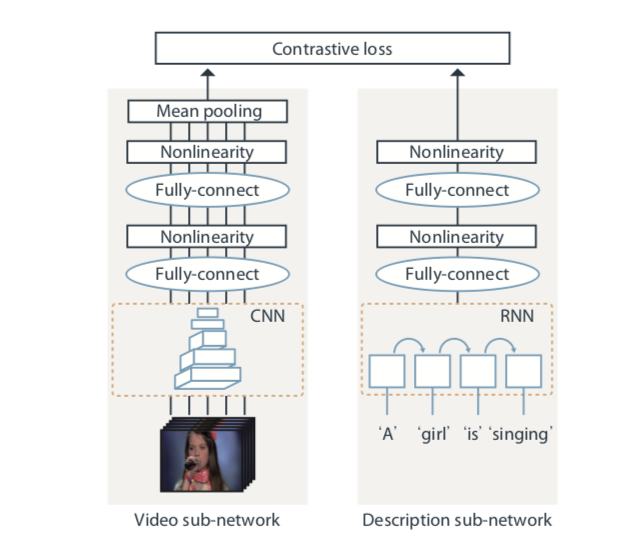
\includegraphics[width=0.5\textwidth]{P1Arch}
				\caption{Deep Semantic Architecture}
				\label{fig:p1arch}
			\end{figure}
			
			
			\subsection{Major Ideas}
				 This paper discusses creating of video summaries using uniformly extracted video segments.
				 
				 Current video suggestion systems according to the paper, \cite{otani_2016_video}, suggest videos based on video metadata, like title, user tags, descriptions, and thumbnails. This is primarily up to the user to specify them.

				As a result if the metadata is misleading, it can lead to completely wrong predictions, as the content of the video is disregarded in current prediction systems.
				
				Further they point to many alternatives that make use of low level visual features that cannot handle various concepts except a predefined set of concepts. Further, videos in real life tend to be of a varied nature, 
				
			\subsection{Input, Processing and Outputs}
				
				\textit{\underline{Input}}
					\begin{itemize}
						\item This uses a temporal sliding window, where the window is shifted by 1 second. 
						\item Each segment, \(V\) was re-sampled at 1 frame per second, so \(V\) has five frames. Thus the video segments run at 1 frame per second. 
						\item In comparison, most modern videos have anywhere between 24 (cinematic) to 60 frames per second (handheld video). Even higher framerates are possible with top of the smartphones and high end video recorders.
					\end{itemize}
				\textit{\underline{Processing}}
					
					The processing pipelined implemented is a DNN, a Deep Neural Network, which utilizes two sub-networks to map a video and its description to a common semantic space and jointly train them using a large-scale dataset.
					
					This video sub-network is a CNN, while the description network is an RNN network. Both these networks are mapped down to a common semantic space and trained using contrastive loss (this method of loss is a distance based loss instead of a error based loss function)
					\begin{align}
						loss(X_n, Y_n) &= t_nd(X_n, Y_n) + (1 - t_n) max(0, \alpha - d(X_n, Y_n))\\
						t_nd &= 1,\ if\ (X_n,Y_n) > 0 \\
						t_nd &= 0,\ otherwise
					\end{align}
					\(d(X_n, Y_n)\) is the squared Euclidean distance between Xn and Yn.
					
					The video sub-network is a modified version of VGG10, modified in order to fit this problem better. A fully connected classification layer has been replaced with two fully connected layers with \texttt{tanh} activation and finally using a mean pooling layer.
					
					Further, the text network uses a Skip-Thought Vector design proposed by Kiros \textit{et al.} \cite{Kiros_2015}
					
				\textit{\underline{Output}}
				
					Visualizing the 2D plot of deep features from a video shows that similar segments are closer in the semantic space and thus applying the solution to the k-medoids problem. This implemented using a parameter, K, that represents the length of the video summary required
					
					Given the set of deep features extracted, k-medoids thus finds and returns the subset of video segments, S, that minimizes:
					
					\begin{align}
						F(S) = \sum_{X\in X}min_{s\in S}||X-S||^2
					\end{align}
				Where the optimal subset is 
					\begin{align}
						S^* = argmin_SF(S)
					\end{align}
					
\section{Content Summarization with content-based Recommender System \texorpdfstring{\cite{jiang_2019_comprehensive}}{}}
%			\begin{mdframed}
%				\textbf{Paper Title: }\textit{Comprehensive video understanding: Video summarization with content-based video recommender design}
%			\end{mdframed}
	\begin{figure}[ht]
	\centering
		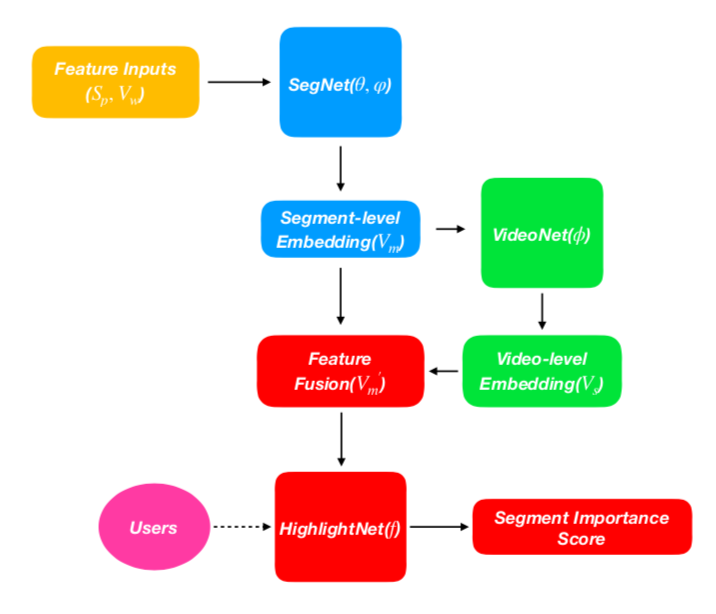
\includegraphics[width=0.5\textwidth]{P2Arch}
	\caption{Recommender Based Architecture}
	\label{fig:p2arch}
    \end{figure}
	
    \subsection{Major Ideas}
    	This paper posits that one of the main challenges in video summarization is with regards to subjectivity, different people may have different selections on what makes an important segment for a video.
    	
    	Key Ideas tackled in this paper are (verbatim from the paper):
    	
    	\begin{enumerate}
    		\item Unifying various inputs on different semantic levels to one framework by formatting video summarization into a recommender problem.
    		\item Developing an algorithm that models independent segments and segment sequence (whole video).
    		\item Extend the summarisation framework with self-supervised learning and data augmentation to deal with the lack of labelled data. (This is a valuable contribution as it enables the system to learn with data that would be more common in real life.)
    	\end{enumerate}
	
    \subsection{Input, Processing and Outputs}
    	
    	\textit{\underline{Input}}
    	
    		This problem models the video summarization task as a video recommendation system wherein each segment is treated as an entity to "recommend". 
    		
    		The input is a set of video segments and the target importance score of each segment.
    		
    	\textit{\underline{Processing}}
    	
    		This uses three subnetworks to learn multiple functions in order to facilitate prediction. 
    		
    		\begin{align}
    			L(f) = L(f(\varphi(\theta(S_p),V_w) \oplus\phi(\varphi(\theta(S_p),V_w))))
    		\end{align}
    		
    		The three subnetworks,
    		
    		\begin{enumerate}
    			\item SegNet will learn \(\theta\) and \(\varphi\)
    			\item VideoNet will learn \(\phi\)
    			\item HighlightNet will learn f
    		\end{enumerate}
    		
    		The video segments are also shuffled often to ensure that the correct segments are determined without focussing on when it occurs in the video.
    		
    	\textit{\underline{Output}}
    
    		By training various models (ResNet50, ResNet152, GoogleNet) on various datasets (ImageNet, and CoView2019), they propose a table comparing the performance.
    		
    		All of the models perform comparably, with their summary score in the range of 80.83 to 81.81. 
			
\section{TruNet: Story Preserving Truncation \texorpdfstring{\cite{yang_2019_trunet}}{}}
    \begin{figure}[ht]
    	\centering
    		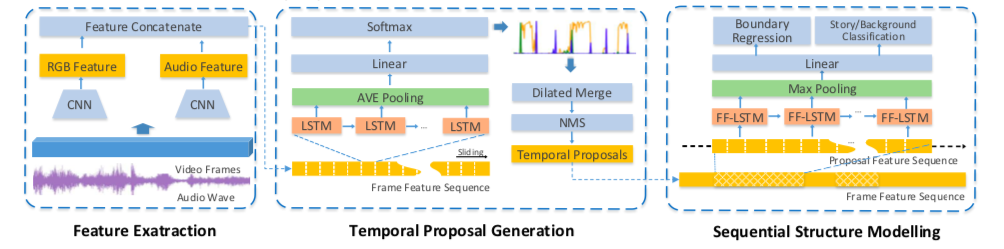
\includegraphics[width=\textwidth]{P3Arch}
    	\caption{TruNet Architecture}
    	\label{fig:p3arch}
    \end{figure}
    			
    \subsection{Major Ideas}
    	This paper points out that although much progress has been made in video highlight detection and video summarization, many of the them focus on producing a coherent whole story in the final combined highlight and there is no requirement of an unbroken story to each sub-video.
    	
    	They develop a large dataset called TruNet, with 1470 videos and a total of 2101 hours of content. The average video length is longer than one hour.
    	
    	These videos are from a variety of sources, like talk shows, TV shows, and reality shows.
    	
    	Their contribution is threefold:
    	
    	\begin{enumerate}
    		\item Introduction of a new practical problem in video truncation
    		\item Collection and annotation of a new large dataset for studying this problem, which can become a complementary source to existing video datasets
    		\item Proposal of a baseline framework that involves a new temporal proposal generation module and a new sequence modeling module, with better performance compared to traditional methods.
    	\end{enumerate}
    
    \subsection{Input, Processing and Outputs}
    	
    	\textit{\underline{Input}}
    	
    		\begin{itemize}
    			\item The paper proposes a custom dataset called the TruNet. On the other hand, the ActivityNet, even though it has more videos, the length of videos is very small, averaging at 2 minutes.
    			\item TruNet proposed by the paper has an average video length of 80 minutes.
    			\item This data is sourced from a wide varying range of content, including talkshows, tv shows, and reality shows.
    		\end{itemize}
    		
    	\textit{\underline{Processing}}
    	
    		The processing methodology is two fold. 
    		
    		\begin{enumerate}
    			\item \textbf{Boundary Aware network:} This is a novel network that takes in 7 consecutive frames as an input to an LSTM and uses the output as an input to a MaxPooling layer and finally a linear layer. \\ It outputs the probabilities of whether these are within the “story” (or the summary),  or background. \\ It also outputs the Story beginning boundary probability and Story ending boundary probability.
    			\item \textbf{FF-LSTM:} For learning, they stack multiple traditional LSTM layers with skip connections running between them. This is called the Fast Forward LSTM (FF-LSTM) \\ These added connections have no non-linear activations nor recurrent computations. Thus, information is propagated easily. \\ Finally a MaxPooling layer is used to average the outputs.
    		\end{enumerate}
    		
    		After computing the intersection over unions (IoU). If \(<\)0.3 then the sample is negative, and if \(>\)0.7 the sample is a positive sample.
    		
    		The BAN network is trained using SGD with momentum 0.9, epoch number 70, decay at 0.0005 and a mini batch size of 256 on four K40 GPUs.
    		
    	\textit{\underline{Output}}
    		For evaluation purposes, the paper computes a mean average precision (mAP) value at three different IoU thresholds, \{0.5,0.7,0.9\}
    		
    		A comparison has been done with state of the art video summary methods, \textbf{vsLSTM} and \textbf{HD-VS}.
    		
    		For different values of the IoU thresholds, \(\alpha\), they showcase that that their model performs consistently better than their alternatives w.r.t. to the mAP values.\cite[Page 8]{yang_2019_trunet}
    		
% \section{Video Summarization and Scene Detection
% by Graph Modeling \texorpdfstring{\cite{graph}}{}}
%     \begin{figure}[ht]
%     	\centering
%     		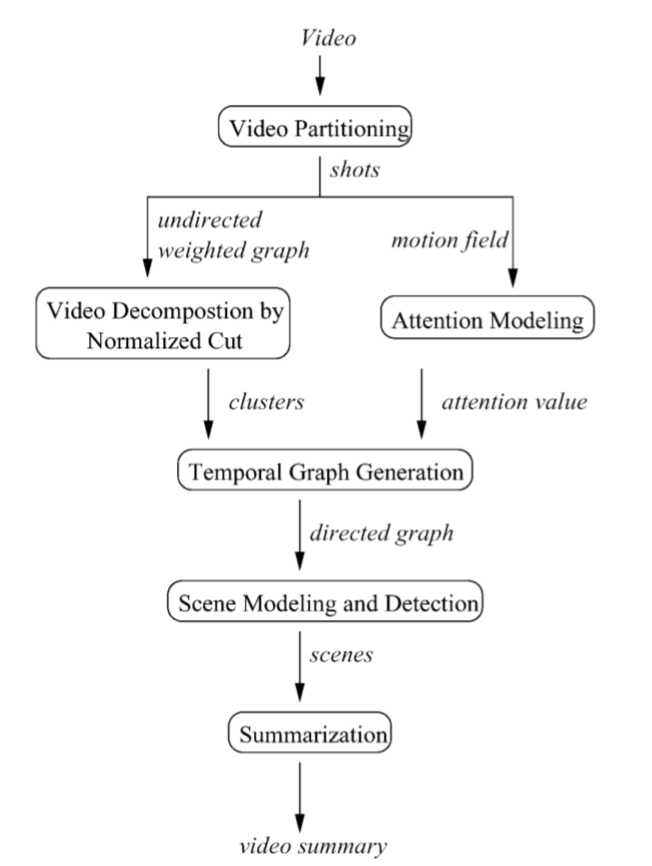
\includegraphics[width=0.4\textwidth]{Ngo}
%     	\caption{Architecture}
%     	\label{fig:ngo}
%     \end{figure}
    			
%     \subsection{Major Ideas}
%         The work in \cite{graph} summarizes video based on entropy, perceptivity and skim ratio. 
        
%         The video is depicted as a temporal graph and this graph is sliced into video clusters by using the normalized cut algorithm.
        
%         These video clusters that are temporally partitioned contains a series of shots with similar visual content. Further, an adaptive keyframe selection and construction scheme is used to select an optimal keyframe from each cluster. 
        
%         This approach takes into account the motion of the objects and the visual setting as a key factor for summarization and excludes captions and spoken text which is expected to reveal semantic details. 
        
%         Results state that with a 75\% cut-off from the original content, 20\% of the information is lost. 
		
%     \subsection{Input, Processing and Outputs}
    	
%     	\textit{\underline{Input}}
    	
%     		\begin{itemize}
%     			\item
%     		\end{itemize}
    		
%     	\textit{\underline{Processing}}
    		
%     		\begin{enumerate}
%     			\item
%     		\end{enumerate}
    		
%     	\textit{\underline{Output}}
    		